\clearpage
\subsection{Subsystem 2: Power Management}

% Subsystem Diagram
\subsubsection{Subsystem Diagrams}
\begin{figure}[h]
    \centering
    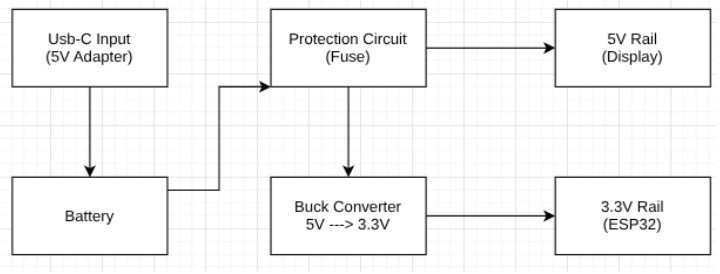
\includegraphics[width=16cm]{images/Power/BlockDiagram-power.jpg} % Change the picture
    \caption{Subsystem Block Diagram}
\end{figure} % If your subsystem is more coding, change it to activity diagram

% Specifications
\subsubsection{Specifications}
\begin{enumerate}
    \item {Input Voltage: 5 V from USB-C adapter.}
    \item {Backup Source: 3.7 V Li-ion battery (at least 8000 mAh)}
    \item {Output Rails:}
    \item {5 V for Display (load up to 3 A)}
    \item {3.3 V for ESP32 (load up to 1 A)}
    \item {Voltage Accuracy: ± 5 \%}
    \item {Average Power Consumption: < 8 W}
    \item {Efficiency: 85\% for buck conversion; 80\% charge/discharge.}
    \item {Protection: fuse (3 A hold)}
    \item {Thermal Limit: surface temperature under 60 °C under full load.}
\end{enumerate}

% Subsystem Interactions
\subsubsection{Subsystem Interactions}
\begin{enumerate}
    \item {With Processing Subsystem (Zeke): Provides regulated 3.3 V rail to ESP32}
    \item {With Display Subsystem (David): Delivers 5 V rail and handles power demand spikes during high-brightness operation.}
    \item {With PCB Integration (Zeke and Joshua): Power traces routed centrally from power management module on PCB, decoupling capacitors placed near load headers to reduce noise}
    \item {With Networking Subsystem (Juan): Shares 3.3 V supply for network module and provides stable voltage during transmit peaks.}
\end{enumerate}

% Core ECE
\subsubsection{Core ECE Design Tasks}
\begin{itemize}
    \item \textbf{ECE 25500}: Electronic Devices and Design Lab: Used to design buck-boost converter and protection circuits
    \item \textbf{ECE 27000}: Digital Systems: Interfaces battery and power-good signals with ESP32 logic pins
    \item \textbf{ECE 36900}: Power Electronics: Guides design of buck and buck-boost stages and load sharing
    \item \textbf{ECE 49595}: Embedded Hardware Design: Applied to joint PCB work with Zeke
\end{itemize}

% Schematics
\subsubsection{Schematics}
[Type here \textbf{DD2+}]
\begin{figure}[h]
    \centering
    
\includegraphics[width=16cm]{images/white.png} % Change the picture
    \caption{[Schematic Name]}
\end{figure} % If your subsystem is more coding, change it to psudo code

% Parts List
\subsubsection{Parts}
\begin{itemize}
    \item USB-C 5 V input module
    \item Li-ion battery pack (3.7 V, 8000 mAh)
    \item Buck-boost regulator IC (for 3.3 V and 5 V rails)
    \item Battery charging IC (USB-C PD or simple Li-ion charger).
    \item Basic protection devices (fuse, MOSFET switch, TVS diode).
    \item (Optional) Solar panel (5–20 W) + MPPT controller IC.
\end{itemize}
\subsubsection{Finalized Parts}
\begin{itemize}
    \item USB-C input controller: STUSB4500 (PD sink, 5 V mode)
    \item Buck-boost regulator: TI TPS63070 (3.3 V / 5 V output from battery or adapter)
    \item Battery charging IC: TP4056 (simple Li-ion charger for 5 V input)
    \item Li-ion battery pack: 3.7 V 8000 mAh flat pack with PCM protection
    \item Fuse: resettable polyfuse (3 A hold)
    \item TVS diode: SMBJ5.0A (for transient suppression)
    \item MOSFET switch: P-channel AO3407A (for reverse protection and load control)
    \item Connectors / Headers: keyed 5 V and 3.3 V output headers with test pads
\end{itemize}
% Algorithm
\subsubsection{Algorithm}
\begin{itemize}
    \item Initialization: detect input source (USB-C present or battery only).
    \item If USB-C is present: supply system load directly and charge battery at regulated current.
    \item If USB-C is removed: automatically switch to battery through PowerPath MOSFET (ideal-diode behavior).
    \item Monitor: ESP32 reads battery voltage and power-good signal periodically.
    \item Low-voltage event: ESP32 alerts display and reduces brightness to conserve power.
\end{itemize}

% Theory of Operation
\subsubsection{Theory of Operation}
The power management subsystem accepts a 5 V input from a USB-C adapter as its primary source. 
When connected, the charger IC diverts current both to the system load and to the battery for charging. 
A buck-boost converter regulates voltage for both 5 V and 3.3 V rails regardless of whether the system is running on the adapter or battery. 
If the adapter is unplugged, the PowerPath MOSFET automatically connects the battery to the load without noticeable interruption (< 100 ms). 
Protection devices (fuse and TVS diode) guard against short circuits and voltage spikes. 
The ESP32 monitors the battery status and can display charging or battery mode indicators.
% Specification Measurement
\subsubsection{Specifications Measurement}
[\textbf{DD3+} Every specification here should match the specification above. ]
\begin{enumerate}
    \item {[Copy specification here. ]} \\
          {[Explain the specification here. Add photoes if necessary. ]}
\end{enumerate}

% Standards
\subsubsection{Standards}
\begin{itemize}
    \item \textbf{USB-C Power Delivery Specification}: ensures safe and standard input power.
    \item \textbf{IEEE 1625}: covers battery system reliability for portable electronics.
    \item \textbf{UL 2054}: safety standard for rechargeable batteries in consumer devices.
    \item \textbf{IEC 61215}: (Optional solar) performance and reliability for PV modules.
\end{itemize}
